%************************************************
\chapter{Design}\label{ch:design} % $\mathbb{ZNR}$
%************************************************
As stated in the introduction (\autoref{ch:introduction}), the research question is the following: ``How can the cost and waste monitoring of a Cloud Computing application be offered in a scalable manner?''. In order to investigate the characteristics of the solution for monitoring a Cloud Computing application, it is important to determine the requirements beforehand. The architectural requirements lead to a proposed architecture. The pricing model leads to specific utilization requirements, which will on their turn be used for waste requirements. The waste requirements will lead to the construction of three algorithms. These will be evaluated in \autoref{sec:optimal_approach} and the optimal approach will be chosen.

\section{Architectural requirements} \label{sec:architectural_req}
As this research is the successor of the work: `Visualizing Computational Waste in Cloud Computing' by A. Spina \cite{spina}, there is some similarity with his architectural requirements. However, his architecture is based on a solution for which a probe collects data from monitored instances, and an aggregator that represents this data into a human-readable format. Relevant requirements are:
\begin{itemize}
    \item The solution should be functional across command cloud providers.
    \item The data should be considered sensitive and secured accordingly.
    \item The solutions should be configurable, but easy to use.
    \item The solution should strike a balance between efficiency and effectiveness.
    \item The solution should collect utilization statistics on the monitored system. 
\end{itemize}

\noindent
In \cite{aceto2013cloud} a number of properties are mentioned. These apply to a distributed monitoring system, and are therefore applicable to the desired solution. The most important properties are:
\begin{itemize}
    \item Scalability: a monitoring system is scalable if it can cope with a large number of probes.
    \item Elasticity: a monitoring system is elastic if it can cope with dynamic changes of monitored entities, so that virtual resources created and destroyed by expansion and contraction are monitored correctly.
    \item Adaptability: a monitoring system is adaptable if it can adapt to varying computational and network loads in order not to be invasive.
    \item Timeliness: a monitoring solution is timely if detected events are available on time for their intended use.
    \item Autonomicity: an autonomic monitoring solution is able to self-manage its distributed resources by automatically reacting to unpredictable changes.
    \item Accuracy: a monitoring system is accurate when the measures it provides are accurate, i.e. they are as close as possible to the real value to be measured.
\end{itemize}

\noindent
Both lists with requirements above are relevant, and the desired solution should be able to meet all these properties. For the implemented solution, the decision has been made to monitor only Docker containers, as this provides a way of abstracting a certain deployment. Therefore, the underlying operating system is insignificant. This ensures that the solution will be functional across all OS's that are capable of running Docker containers. 

\section{Architecture} \label{sec:architecture}
As mentioned in \autoref{sec:related_technologies}, the proposed architecture uses state-of-the-art open-source technologies. Several design patterns have been evaluated, such as a Client-Server network and a peer-to-peer network \cite{coulouris2005distributed}. The latter is considered more scalable, as the number of resources grow with the number of nodes. Additionally, a peer-to-peer system does not have a single point of failure. Therefore, this system is desired over a client-server network. However, as the data is stored in a Prometheus database, and this cannot operate in a peer-to-peer system, another solution is needed. Using the federation technique of Prometheus \cite{prometheus_federation}, the decision has been made for a hierarchical network. This proposed network consists of only one root, a number of supernodes, and optional a number of nodes.\\

\noindent
An architectural overview of the three node types, as well as the technologies that are included, can be found in \autoref{fig:architecture}. Several processes are listed in bold as this denotes a custom created process. The only difference between a node and a supernode is the Prometheus database. Furthermore, the root is only used to visualize the collected metric data in the Grafana dashboard. Each node type is shortly described below.

\begin{figure}
    \centering
    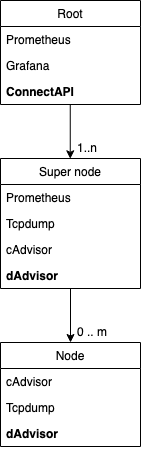
\includegraphics[width=0.3\textwidth]{gfx/architecture.png}
    \caption{Architectural overview}
    \label{fig:architecture}
\end{figure}

\subsection{Root} \label{sec:root}
The root is a single access point for the displaying the obtained results. The corresponding Prometheus database is dynamically configured, such that it scrapes data from all the super nodes deployed in the system. 
In order to successfully deploy the entire system, the root needs to be deployed first, as it provides an access point for the nodes as well. This access point is implemented in the connect API and further described in \autoref{sec:impl-root}. The connect API distributes the available nodes over the available super nodes.

\subsection{Super node} \label{sec:supernode}
As explained before, there is only a slight difference between a node and a super node, as the latter deploys Prometheus. This database is automatically configured such that is scrapes from a set of nodes (as received from the root). The metrics that a super node collects are the same as for a node and are therefore described in the following section.

\subsection{Node} \label{sec:node}
The node consists of three processes. Resource metrics (i.e. CPU and memory) are collected using the cAdvisor process and internet packets are collected using Tcpdump \cite{tcpdump}. This data is collected using the dAdvisor process, which acts as an aggregator. This process ensures that the data is correctly formatted, and makes it available for Prometheus.

\subsection{Conclusion}
The architecture is proposed in \autoref{sec:root}, \autoref{sec:supernode} and \autoref{sec:node}. According to the Prometheus documentation, this architecture can scale up to ''tens of data centers and millions of nodes`` \cite{prometheus_federation}. Therefore, it provides a scalable way of monitoring the infrastructure. However, the dAdvisor component restricts the scalability a bit. This analysis is described in \autoref{sec:exposing_data}.

\section{Pricing model} \label{sec:pricing}

Another design decision is to propose an accurate pricing model for estimating the price of a VM based on its resources.
This pricing model will then be used with the consumed resources to estimate the cost of running a container.
Different schemes and models exist for different service providers \cite{bulla2014cloud}. However, the most common model employed in cloud computing is the ``pay-as-you go'' model. Customers pay a fixed price per unit of use. Amazon\footnote{\url{https://aws.amazon.com/}}, considered the market leader in cloud computing, utilizes such a model by charging a fixed price for each hour of virtual machine usage. 
Another common scheme employed by these leading enterprises is the ``pay-per-use'' model. A customer pays for the amount of bandwidth or storage utilized.\\

\noindent
The authors of \cite{mazrekaj2016pricing} provide an overview of the pricing model for the three most popular public cloud providers:
\begin{itemize}
    \item \textbf{Google Cloud / App engine: }Charges on monthly basis, per user, and pricing is based on hourly basis.
    \item \textbf{Amazon Web Services / Elastic Compute Cloud (EC2): }It allows for the reservation of units.
    \item \textbf{Microsoft Azure: }Charges on monthly basis, depending on the number of transactions, and on a monthly basis for their database subscription.
\end{itemize}

Using the literature above and the Google Compute Engine Pricing\footnote{See \url{https://cloud.google.com/compute/pricing}. They bill each vCPU and each GB of memory on Compute Engine separately.}, we propose a pricing model $p$ by the following formula:

\begin{equation} \label{eq:p}
p(t) = n_\text{CPU}(t) * p_\text{CPU} + n_\text{memory}(t) * p_\text{memory} + n_\text{network}(t) * p_\text{network}
\end{equation}

\noindent
Where $n_\text{CPU}(t)$ is the amount of CPU cores requested per hour on a specific host over time $t$. For example, if 2 CPU cores are requested for 3 hours, then $n_\text{CPU} = 6$. $p_\text{CPU}$ is the price per CPU per hour. The same notion applies to $n_\text{memory}(t)$ and $p_\text{memory}$. $n_\text{network}(t)$ represents the amount of outgoing network in GB over time $t$. Note that all cloud providers only charge for network traffic flowing out of their system, and not for communication between internal services. $p_\text{network}$ is the price of this outgoing network per GB.\\

\noindent
The pricing model $p(t)$ can be used to compute the actual cost by summing over all time instances $t$: $c_\text{actual} = \sum_t p(t)$. This cost model can be split into \textit{effective cost}, meaning the cost for used resources, and \textit{waste cost}, a cost model for unused resources. This implies that $n_\text{used CPU} + n_\text{unused CPU} = n_\text{CPU}$. When it comes to the network cost, all the external network is used, and therefore there is no network cost modelled in $c_\text{waste}$. 

\begin{equation} \label{eq:cost_and_waste}
\begin{split}
c_\text{effective} &=  n_\text{used CPU} * p_\text{CPU} + n_\text{used memory} * p_\text{memory} + n_\text{network} * p_\text{network} \\
c_\text{waste} &=  n_\text{unused CPU} * p_\text{CPU} + n_\text{unused memory} * p_\text{memory}
\end{split}
\end{equation}

\noindent 
Although not stated, the $c_\text{effective}$ and $c_\text{waste}$ are computed for a specific time $t$ and then summed to get the total $c_\text{effective}$ and $c_\text{waste}$. There are different prices per cloud provider, and it even differs per cloud provider itself, as the cloud provider might provide a discount for longer use. It is therefore not desired to implement a fixed price. Instead, the solution provides the possibility to dynamically change the prices, such that the total cost can be affected. 

%However, to provide an easy-to-use solution, the following default prices are used:
%\begin{itemize}
%    \item $p_\text{CPU}$: USD 0.021925 per hour per CPU per host.
%    \item $p_\text{memory}$: USD 0.002938 per hour per GB memory per host.
%    \item $p_\text{network}$: USD 0.10 per GB of network traffic going out of their system.
%\end{itemize}


\section{Utilization requirements} \label{sec:util_req}
The CPU and memory are resource metrics that are specified per Docker container. They are either used, or unused as described in \autoref{sec:pricing}. In this section, the used resource (which is either the CPU or memory\footnote{Note that the network resource is excluded, as this is all \textit{effective cost}. Therefore, there is no distribution of the network for the \textit{waste cost}.}) is denoted by $u_i$, which represents the percentage of used resource for a specific container. We assume in this model that $n_\text{used CPU} = n_\text{cpu} * \sum_{i=1}^n u_i$. Additionally, $n_\text{unused CPU} = n_\text{cpu} * \sum_{i=1}^n w_i$. The same formulas can be specified for the memory resource.\\

\noindent
For a specific node, the sum of these metrics over all containers is denoted as the total utilization. For these utilization values, there are a few restrictions, which are mathematically stated below.

\begin{itemize}
    \item $0 < u_i \leq 1$ for $1 \leq i \leq n$: Every container on a node utilizes a value between $0$ (exclusive) and 1 (inclusive). The desired solution will also be a running container, but the utilization is filtered out of the collected utilization values, such that the monitoring solution only collects data about the deployed system.
    \item $\sum_{i=1}^n u_i \leq 1$: The total utilization of containers for a given host cannot utilize more than 100\%. And with the previous requirement, its lower-bound is 0 (exclusive). As the total waste is computed as $1 - \sum_{i=1}^n u_i$, it can be concluded that the waste is bounded by 0 (inclusive) and 1 (exclusive).
\end{itemize}



\section{Waste requirements} \label{sec:waste_requirements}
There are several ways in which the utilization values can be used to compute the waste. In this, the following four properties are used for finding an optimal waste distribution. The waste distribution is computed per node, as is the same for the cost requirements above.
\begin{enumerate}
    \item \textbf{$\sum_{i=1}^n w_i = 1 - \sum_{i=1}^n u_i $}: The sum of the elements of the waste and the sum of the elements of the utilization values should sum up to 1, as it implies that a resource is either used (this is $u$) or being wasted (this is $w$).
    \item \textbf{$w_i \geq 0$} for $1 \leq i \leq n$: The waste of every certain container is non negative. Thus, it is impossible for a container to have a negative waste. As the waste distribution is used for computing the amount of money wasted, this would imply that money is being earned, while running a certain container.
    \item \textbf{$\max w_i \Rightarrow \min u_i$}: The container that utilizes the most resources, should be responsible for wasting the least amount of resources. This property implies that the order of containers from lowest utilization to highest utilization is the same as the order of containers from highest waste to lowest waste. 
    \item \textbf{$u_i = u_j \Rightarrow w_i = w_j $}: If two containers utilize the same amount of resources, than they should also waste the same amount of resources. The inverse does not necessarily hold. If two containers utilize both a different amount of resources, than it is not guaranteed that they have a different amount of waste.
\end{enumerate}

\noindent
The following section contains several approaches for computing the waste distribution. These three approaches are evaluated in \autoref{sec:optimal_approach}.

\section{Approaches for computing the waste distribution} \label{sec:approaches}
In this section, the following three waste distributions will be evaluated: uniform distribution, linear inverse distribution and proportional inverse distribution. They are all described in a different subsection below.

\subsection{Uniform distribution} \label{sec:equal}
Using a uniform distribution, the waste is the same for every container on a certain host, i.e. $w_1 = w_2 = \dots = w_n$. The idea behind this approach is that a set of containers together wastes the same part of the host and therefore the waste should be distributed over every container in a fair manner. This approach can be computed by the following formula:
\begin{equation}
w_i = \frac{1 - \sum_{i=1}^n u_i}{n}
\end{equation}

\subsection{Linear inverse distribution} \label{sec:linear}
This distribution computes a higher waste for a container that utilizes less, and can be computed by the following formula:
\begin{equation} \label{eq:linear}
w_i = \frac{1}{n} - u_i
\end{equation}
However, it is easy to see that \autoref{eq:linear} returns a negative value if $u_i > \frac{1}{n}$ (contradicts property 2). Therefore, this formula can be replaced by the following formula:
\begin{equation}\label{eq:heuristic}
w_i = \begin{cases}
\frac{1}{n} - u_i & \text{if } u_i \leq \frac{1}{n}\\
0                 & \text{otherwise}
\end{cases}
\end{equation}
This yields another problem, as it is not guaranteed that property 1 holds. In fact, property 1 will fail, if there exists a $j$ for which $u_j > \frac{1}{n}$ (the function returns the \textit{otherwise}-case). Therefore, a simple formula can be used to restore property 1. Note that $u = \sum_{i=1}^n u_i$ and $w = \sum_{i=1}^n w_i$ and needs to be computed before the first $w_i$ is updated.
\begin{equation} \label{eq:update}
w_i \leftarrow w_i * \frac{1-u}{w}
\end{equation}
An example for $n = 2$ is the following distribution $u_1 = 0.6$ and $u_2 = 0.3$. Using \autoref{eq:heuristic}, the following values are found $w_1 = 0$ and $w_2 = 0.2$. However, since property 1 doesn't hold, $w_2$ is updated to $0.1$. The entire algorithm for this approach is formulated in Algorithm \ref{alg:linear}.

\begin{algorithm}
    \caption{Compute the waste based on the linear inverse distribution}\label{alg:linear}
    \begin{algorithmic}[1]
        \Procedure{computeWaste}{$u_1, u_2, \dots, u_n$}
        \For{$i \gets 1 \dots n$}
        \State $w_i\gets \max(\frac{1}{n} - u_i,~0)$
        \EndFor
        \State $u\gets \sum_{i=1}^n u_i$
        \State $w\gets \sum_{i=1}^n w_i$
        \If{$u+w \neq 1}$
        \For{$i \gets 1 \dots n$}
        \State $w_i\gets w_i * \frac{1-u}{w}$
        \EndFor
        \EndIf
        \State \textbf{return} $w_1, w_2, ..., w_n$
        \EndProcedure
    \end{algorithmic}
\end{algorithm}


\subsection{Proportional inverse distribution} \label{sec:proportional}
This distribution uses the idea that the product of the utilization and the waste distribution should be constant for every container. 
The formula is therefore: $w_i * u_i = c$ for an unknown value of $c$. This implies that if a certain container utilizes a high amount of resources, its corresponding waste must be a low number. By default, a container has no resource constraints and can use as much of a given resource as the host’s kernel scheduler allows \cite{docker:resource}.
The $c$-value is constant across all containers on a specific host, which leads to the general formula: 
\begin{equation} \label{eq:constant}
w_1 * u_1 = w_2 * u_2 = \dots = w_n * u_n
\end{equation}
However, in case of $n = 1$, there is no equation possible. In this case, the waste can directly be computed using property 1, and thus $w_1 = w = 1 - u_1$.\\

\noindent
In general (for $n \geq 2$), \autoref{eq:constant} results in $n-1$ unique equations. However, this set of equations cannot be solved, as there are $n$ variables unknown ($w_1$ to $w_n$). But property 1 can be used to generate $n$ unique equations. For example, for $n=3$ the following equations needs to be solved:
\begin{equation}\label{eq:linear3}
\begin{split}
w_1 & u_1 - w_2 * u_2 &= 0 \\
w_1 & u_1 - w_3 * u_3 &= 0 \\
w_1 + w_2 + w_3 &= 1 - u_1 - u_2 - u_3
\end{split}
\end{equation}
This system of linear equations can be represented by a matrix equation of the form $Ax = b$:
\begin{equation} \label{eq:matrix}
\begin{split}
A x &= b\\
\begin{bmatrix}
u_1 & -u_2 & 0    \\
u_1 & 0    & -u_3 \\
1   & 1    & 1
\end{bmatrix}
\begin{bmatrix}
w_1 \\ w_2 \\ w_3
\end{bmatrix}
&= \begin{bmatrix}0 \\ 0 \\ 1 - \sum_{i=1}^3 u_i\end{bmatrix}
\end{split}
\end{equation}

\noindent
\autoref{eq:matrix} can be generalized for $n$ containers. The matrix $A_n$, as well as vectors $w$ (was $x$ in \autoref{eq:matrix}) and $b$ are expressed below:
\begin{equation} \label{eq:general_matrix}
\begin{split}
A_n &= \begin{bmatrix}
u_1    & -u_2 &       &        & \\
u_1    &      &  -u_3 &        & \\
\vdots &      &       & \ddots & \\
u_1    &      &       &        & -u_n \\
1      & 1    & 1     & \dots  & 1 \\
\end{bmatrix}
\end{split}
\begin{split}
w &= \begin{bmatrix}w_1 \\ w_2 \\ \vdots \\ w_{n-1} \\ w_n\end{bmatrix}
\end{split}  
\begin{split}
b = \begin{bmatrix}
0 \\ 0 \\ \vdots \\ 0 \\ 1 - \sum_{i=1}^n u_i
\end{bmatrix}
\end{split}
\end{equation}

\noindent
Thus, the waste values can be computed by solving $A_n w = b$. 
In general, the following two properties needs to hold to have a unique solution given by $w = A_n^{-1} b$:
\begin{itemize}
    \item \textbf{The matrix is a square}: this holds, as $A_n$ has $n$ rows and $n$ columns.
    \item \textbf{The matrix has full rank (all rows are linearly independent)}: this also holds, as this is how matrix $A_n$ was constructed from the equation in \autoref{eq:linear3}.
\end{itemize}
Therefore, the matrix $A$ is invertible. This also implies that its determinant is non-zero. This also holds and is proven in \autoref{ch:proof}. Thus, $A^{-1}$ can always be constructed, and this implies that $w$ can always be solved.

\section{Optimal approach} \label{sec:optimal_approach}
In the previous section, three approaches for distributing the waste resources over the containers have been proposed.
This section analyses the three approaches according to their complexity and accuracy. 

\subsection{Complexity}
The complexity can be expressed in terms of memory complexity and computational complexity. They are all listed in \autoref{tab:complexity}. The minimal computational complexity is $\mathcal{O}(n)$, as a host runs $n$ containers. Approach 1 has a memory complexity of $\mathcal{O}(n)$, as the result can be stored in the same variable for all containers. Approach 2 has a memory complexity of $\mathcal{O}(n)$, as this algorithm only iterates the utilization values as well. The \textit{Linear inverse distribution} has a computational complexity of $\mathcal{O}(n^3)$ as this is necessary for solving a system of linear equations in the worst case. However, \cite{pan1991complexity} explains that there exists several optimization and thus may be usually be done in $\mathcal{O}(n^2)$.\\

\noindent
As the \textit{Proportional inverse distribution} (\autoref{sec:proportional}) is clearly the worst in terms of memory and computational complexity it can be argued that $n$ is usually not a very large number, as it represents the number of containers for a specific host. According to a survey from 2017 \cite{docker_report}, the median number of containers per host is 10. However, this survey also stated that they have a response with 95 containers per host. In both cases, the waste can be easily computed. On an average machine, computing the waste for for $n = 100$ takes less than 1 millisecond. Given that this needs to be computed only once an hour, all three approaches are sufficient.

\begin{table}
    \centering
    \begin{tabular}{l|r|c|c}
        \textbf{Approach} & \textbf{\#} & \textbf{Memory} & \textbf{Computational} \\ \hline
        Uniform distribution & 1 & $\mathcal{O}(1)$ & $\mathcal{O}(n)$ \\
        Linear inverse distribution & 2 & $\mathcal{O}(n)$ & $\mathcal{O}(n)$ \\
        Proportional inverse distribution & 3 & $\mathcal{O}(n^2)$ & $\mathcal{O}(n^3)$ \\
    \end{tabular}
    \caption{Memory and Computational complexity for the three different approaches}
    \label{tab:complexity}
\end{table}

\begin{table}
    \centering
    \begin{tabular}{|r|r|r|r|r|r|r|r|r|}
        \hline
        \multicolumn{4}{|c|}{\textbf{Utilization}} & \multirow{2}{*}{\textbf{Approach \#}} & \multicolumn{4}{|c|}{\textbf{Waste}} \\ 
        $u_1$ & $u_2$ & $u_3$ & $\sum$ & \multirow{2}{*}{} & $w_1$ & $w_2$ & $w_3$ & $\sum$ \\ \hline
        
        \multirow{3}{*}{0.10} & \multirow{3}{*}{0.15} &  & \multirow{3}{*}{0.25} 
        & 1 & 0.375 & 0.375 & &                            \multirow{3}{*}{0.75} \\
        \multirow{3}{*}{}     & \multirow{3}{*}{}     & & \multirow{3}{*}{}
        & 2 & 0.4 & 0.35 & & \multirow{3}{*}{} \\
        \multirow{3}{*}{}     & \multirow{3}{*}{}     & & \multirow{3}{*}{}
        & 3 & 0.45 & 0.3 & & \multirow{3}{*}{} \\ \hline
        
        \multirow{3}{*}{0.60} & \multirow{3}{*}{0.15} &  & \multirow{3}{*}{0.75} 
        & 1 & 0.125 & 0.125 & &                            \multirow{3}{*}{0.25} \\
        \multirow{3}{*}{}     & \multirow{3}{*}{}     & & \multirow{3}{*}{}
        & 2 & 0 & 0.25 & & \multirow{3}{*}{} \\
        \multirow{3}{*}{}     & \multirow{3}{*}{}     & & \multirow{3}{*}{}
        & 3 & 0.05 & 0.20 & & \multirow{3}{*}{} \\ \hline
        
        \multirow{3}{*}{0.10} & \multirow{3}{*}{0.35} & \multirow{3}{*}{0.35} & \multirow{3}{*}{0.80} 
        & 1 & 0.067 & 0.067 & 0.067 & \multirow{3}{*}{0.20} \\
        \multirow{3}{*}{}     & \multirow{3}{*}{}     & \multirow{3}{*}{} & \multirow{3}{*}{}
        & 2 & 0.20 & 0 & 0 & \multirow{3}{*}{} \\
        \multirow{3}{*}{}     & \multirow{3}{*}{}     & \multirow{3}{*}{} & \multirow{3}{*}{}
        & 3 & 0.127 & 0.036 & 0.036 & \multirow{3}{*}{} \\ \hline
        
        \multirow{3}{*}{0.05} & \multirow{3}{*}{0.05} & \multirow{3}{*}{0.45} & \multirow{3}{*}{0.55} 
        & 1 & 0.15 & 0.15 & 0.15 & \multirow{3}{*}{0.45} \\
        \multirow{3}{*}{}     & \multirow{3}{*}{}     & \multirow{3}{*}{} & \multirow{3}{*}{}
        & 2 & 0.225 & 0.225 & 0 & \multirow{3}{*}{} \\
        \multirow{3}{*}{}     & \multirow{3}{*}{}     & \multirow{3}{*}{} & \multirow{3}{*}{}
        & 3 & 0.213 & 0.213 & 0.023 & \multirow{3}{*}{} \\ \hline
        
    \end{tabular}
    \caption{Several utilization values and the waste values that are computed using the three approaches}
    \label{tab:values}
\end{table}

\subsection{Accuracy} \label{sec:data}
As the previous section has shown that the computational and memory complexity is not significant in choosing the best approach, it is interesting to investigate the difference in their results. This section shows the actual values and whether these can be justified. In order to do so, several utilization distributions have been generated and have been listed in \autoref{tab:values}. This table provides two examples with $n = 2$, and two examples with $n = 3$. In the first row, the waste for all three approaches are approximately equivalent. However, in the second row, the waste varies a lot between the different approaches. It feels unnatural that, if a container utilizes 4 times more than another container, its corresponding waste is the same. Therefore, the computations from the approach described in \autoref{sec:equal} feel to simplistic.\\

\noindent
In the case of $n = 3$, the table provides two examples. It can be observed that the approach describes in \autoref{sec:linear} returns $0$ if the utilization is too high. However, this might also feel unnatural, as there is the notion that every container might be able to reduce its waste. It also needs to be stated that the approach from \autoref{sec:proportional} might seem incorrect as well, as the it is based on the assumption that every container utilizes and wastes the same amount ($u_i * w_i = c$). Although it is required that $u_i > 0$, it can be close to $0$. This leads to the fact that this container utilizes almost every waste, i.e. $w_i \approx \sum_{i=1}^n w_i$.\\

\noindent
Apart from presenting the data in a table, it is also possible to visualize this in a graph. This visualization can be found in Figure \ref{fig:approaches}. It consists of two examples of utilization distributions, each consisting of two utilization values. This visualization should be interpreted by drawing a vertical line from the utilization values to the waste values. For example, in \autoref{fig:approaches:A}, the utilization values in the left most position are $u_1 = 0.2$ and $u_2 = 0$. This results in $w_1 = w_2 = 0.4$ for approach 1, $w_1 = 0.3, w_2 = 0.5$ for approach 2, and $w_1 = 0, w_2 = 0.8$ for approach 3. Using \autoref{fig:approaches:A}, it can be observed how the waste values change if one utilization value remains constant, while the other utilization value increases. In \autoref{fig:approaches:B} it can be observed how the waste values change while one utilization value increases and another decreases. In this figure, the sum of the utilization values remains constant, while it increases in \autoref{fig:approaches:A}.


\begin{figure}
    \subfloat[Example 1]{%
        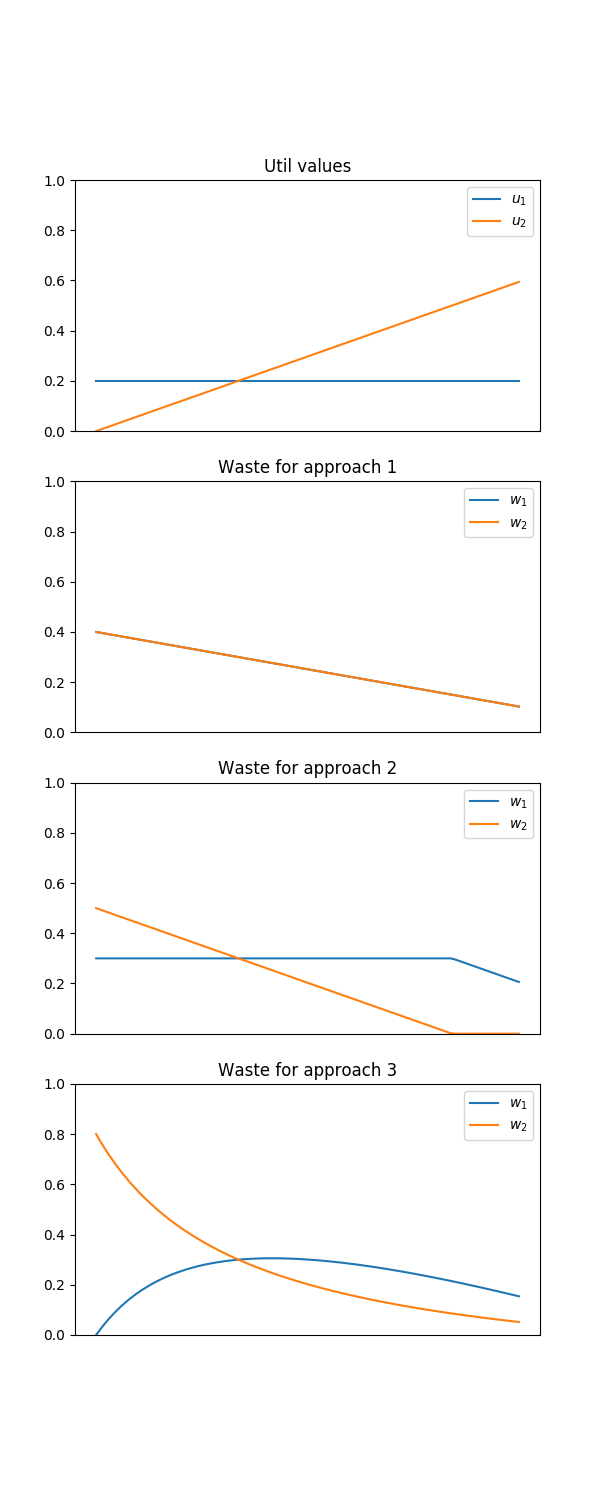
\includegraphics[width=6cm]{gfx/exampleA.png}%
        \label{fig:approaches:A}%
    }\qquad
    \subfloat[Example 2]{%
        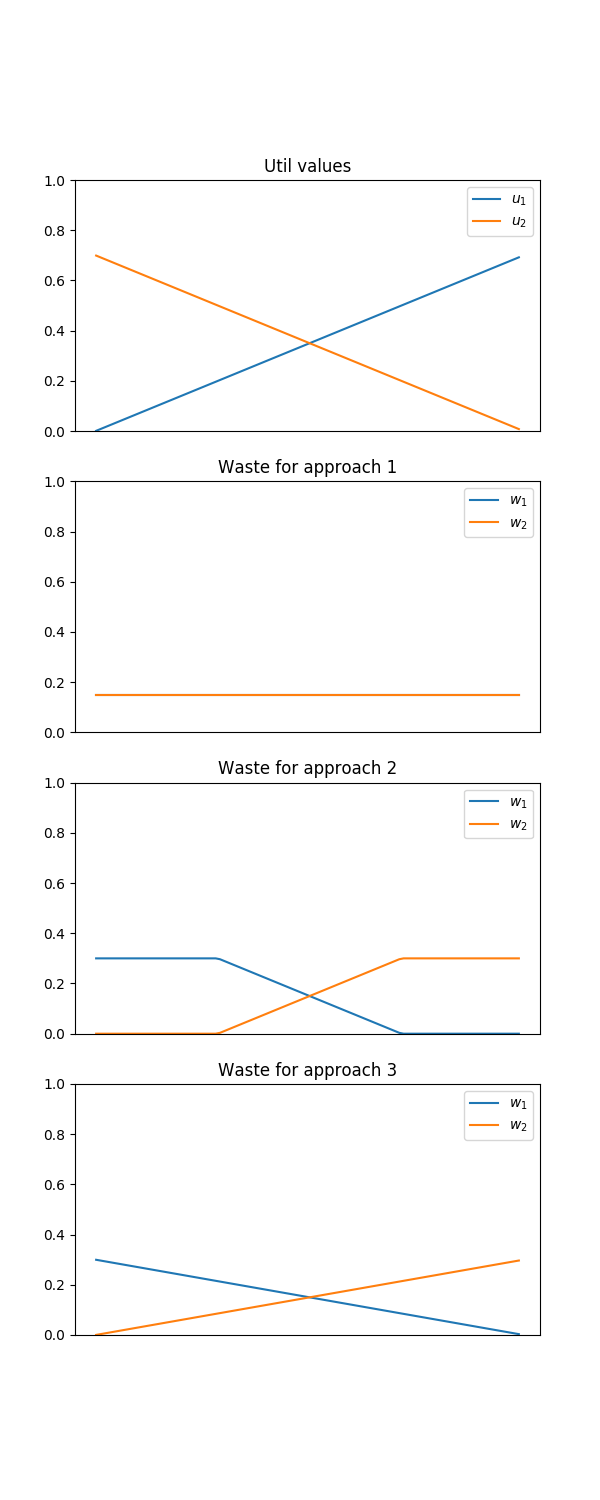
\includegraphics[width=6cm]{gfx/exampleB.png}%
        \label{fig:approaches:B}%
    }
    \caption{Two utilization values and their corresponding waste distribution}
    \label{fig:approaches}
\end{figure}


\subsection{Conclusion} \label{sec:conclusion4}
One of the properties of the utilization values (as stated in \autoref{sec:waste_requirements}) is that $u_i > 0$ for all $i$. However, while deploying the system, it turned out that the utilization of a certain container was zero. In the first two approaches (\autoref{sec:equal} and \autoref{sec:linear}), this is not a problem. However, this is a problem for the last approach (\autoref{sec:proportional}). An example can be seen for $n = 3$ with $u_1 = 0.3, u_2 = 0, u_3 = 0.2$. This results in the waste values: $w_1 = 0, w_2 = 0.5, w_3 = 0$. Therefore, if $u_1 = 0$, then $w_i = 1 - u$.\\

\noindent
In case there are two containers that have a zero utilization, than the waste cannot be computed for the third approach. This is due to the fact that the matrix $A_n$ does not have a full rank anymore (as two rows are the same). This problem can be avoided by adding a small utilization value $\Delta$ to the $u_i$-values that are $0$. This value can then be removed from the corresponding $w_i$ value, to ensure that property 1 still holds. However, as explained in \autoref{sec:data}, the corresponding $w_i$ will be close to $\sum_{j=1}^n w_j$ and will lead to abnormal results. This leads to the conclusion that the \textit{linear inverse distribution} (described in \autoref{sec:linear}) is sufficient for the implementation. Thus, Algorithm \ref{alg:linear} will be used to compute the waste values given the utilization values.

\section{Conclusion}
In \autoref{sec:architecture} a system is proposed that meet the architectural requirements from \autoref{sec:architectural_req}. With this system, the used an unused cost can be modelled on a containerized level. This is model is proposed in \autoref{sec:pricing}. This model is based on several variables, for which some of them are unknown. For resolving the unknown variables, thee algorithms have been proposed in \autoref{sec:approaches}. One of these algorithms is chosen in \autoref{sec:optimal_approach}.